\documentclass{article}

\usepackage[margin=1in]{geometry}
\usepackage{graphicx}
\usepackage{subcaption}
\usepackage[space]{grffile}
\usepackage{latexsym}
\usepackage{amsfonts,amsmath,amssymb}
\usepackage{url}
\usepackage[utf8]{inputenc}
\usepackage{fancyref}
\usepackage{hyperref}
\hypersetup{colorlinks=false,pdfborder={0 0 0},}
\usepackage{textcomp}
\usepackage{longtable}
\usepackage{multirow,booktabs}
%\usepackage{aas_macros}
%\usepackage{aastex_hack}
%Bib stuf
\usepackage{natbib}
\bibliographystyle{abbrvnat}
\setcitestyle{authoryear,open={(},close={)}}
\usepackage{threeparttable}


%\usepackage{minted}
%colors
\usepackage{color}
\definecolor{blue}{rgb}{0.0, 0.0, 1.0}
\definecolor{grn}{rgb}{0.13, 0.55, 0.13}
\definecolor{fulvous}{rgb}{0.86, 0.52, 0.0}
\definecolor{blush}{rgb}{0.87, 0.36, 0.51}
\definecolor{cadmiumorange}{rgb}{0.93, 0.53, 0.18}
\definecolor{byzantium}{rgb}{0.44, 0.16, 0.39}
\definecolor{alizarin}{rgb}{0.82, 0.1, 0.26}

\newcommand{\truncateit}[1]{\truncate{0.8\textwidth}{#1}}
\newcommand{\scititle}[1]{\title[\truncateit{#1}]{#1}}

\begin{document}
\author{D. C. Jacobs}
\title{Signal Loss due to Emperically Estimated Inverse Covariance Weighting}

\date{\today}
\maketitle	

Here I investigate the signal loss one gets from estimating covariance empirically in data under conditions of low number statistics.

Lets keep things simple, our simulated data set is a set of Nchan channels, measured Ntimes on Nbaselines.   Divide our Nbaselines into Ngroups. Within each group compute the weighted data and then measure the power spectrum cross-multiplying between independent groups.  Calculate the power spectrum over many trials drawing different ``eor'' signals each time.  \footnote{``Visibilities'' are simulated here as real numbers to minimize complexity.}  EoR is simulated by drawing random noise, filtering to provide a crude simulation of the way a true sky has only a few independent noise,  and then adding this common signal to each baseline.   Finally the data are filtered again (with the same filter) to reflect the final fringe rate filter performed on the data.
\begin{equation}
X = \textrm{frf}(\textrm{frf}(\textrm{E}) + \textrm{N})
\end{equation}
the dimensions of $X$, and the length scale of the filter are sized to match time and frequency in a typical PSA64 data set.


The power spectrum calculation is pretty basic
\begin{equation}
C = X\cdot X^\mathsf{T}
\end{equation}
Apply the inverse to the data
\begin{equation}
Y = C^{-1}\cdot \textrm{X}
\end{equation}

Sum the weighted data over many draws of noise (equivalent to baseline groups in the paper pipeline). Also sum the inverse weight matrices.
\begin{align}
Y_g &= \sum_i^{N_b} Y_i\\
\textrm{Cinvsum} &= \sum_i^{N_b} C_i^{-1}
\end{align}
where $i$ indexes redundant baselines within groups/different draws of independent noise and simulates the effect of having the input signal be below the noise on every individual sample.

Next, cross multiply between different baseline groups
\begin{equation}
P_{out} = \frac{\sum_{i\neq j} Y_i \cdot Y_j }{\sum_{i\neq j} W_i W_j}
\end{equation}
where $i$ and $j$ index different groups and $W$ is a weight vector formed by summing across the rows of Cinvsum.


Using this method we calculate a number of power spectra for each trial,

The injected power spectrum 
\begin{equation}
P_{in} = E E^\mathsf{T}
\end{equation}

the input noise power spectrum  
\begin{equation}
P_{noise} = < N N^\mathsf{T} >
\end{equation}
where brackets indicate average over baselines and cross multiplication between groups as described above.


The weighted power spectrum output with the injected signal 
\begin{equation}
P_{out} = < X C_X^{-1} C_X^{-1} X^\mathsf{T} >
\end{equation}

as well as the weighted power spectrum output \emph{without} the injected signal, ie the uncorrected power spectrum output from our pipeline.
\begin{equation}
P_{v} = < N C_N^{-1} C_N^{-1} N^\mathsf{T} >
\end{equation}

%\item "foreground" power spectrum (noise realization that is the same on every baseline) $P_{fg}$


The output for each inject value is a large number of trial output power spectrums, over which there is a wide range of losses (near 0 to 100\%).  

\section*{Loss Estimators}

Given a lossy estimator we can formulate multiple slightly different questions:
\subsection*{First estimator: Total Power} 
In this measure we ask: ``What is the output power spectrum for a range of 21cm signal power levels?`` In this measure one sets the weighted power spectrum $P_{meas}$ equal to the total output power spectrum,
\begin{equation}
P_{v} = P_{out} 
\end{equation}
$P_{out}$ includes whatever is in the original data (noise, foregrounds, 21cm signal) as well as the injected 21cm simulation.  The result is plotted in Figure \ref{fig:outvin}

\begin{figure}[bth]
\begin{center}
\begin{subfigure}{0.45\textwidth} \centering
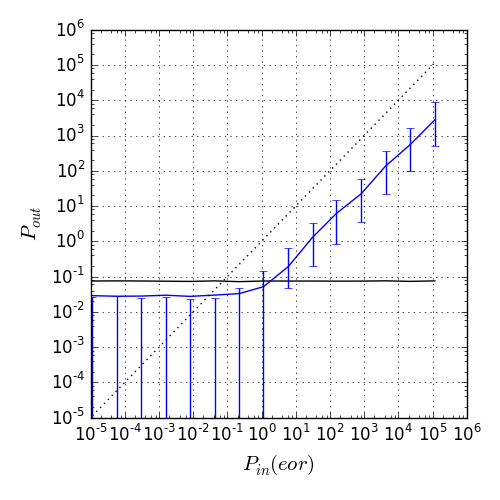
\includegraphics[width=\textwidth]{C_loss_Nlst6_Neor6_fgscale0.001_frf_Pv_wide_PP.png}
     \caption{$P_{out}$ vs $P_{in}$:   Weighted net output power spectrum as a function of injected power spectrum.   Error bars enclose 50\% of the run outputs.}\label{fig:outvin}
   \end{subfigure}
   \begin{subfigure}{0.45\textwidth} \centering
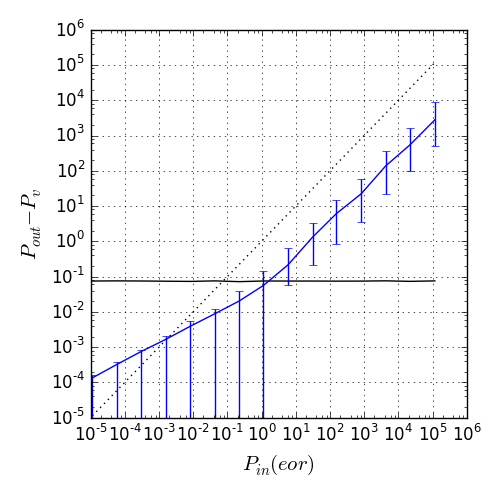
\includegraphics[width=\textwidth]{C_loss_Nlst6_Neor6_fgscale0.001_frf_Pv_wide_sub_PP.png}
     \caption{$P_{out}-P_v$ vs $P_{in}$: Here we make an estimate of the recovered injected power spectrum by    subtracting the weighted power spectrum of the data before the eor simulation is injected.}\label{fig:eorvin}
   \end{subfigure}
\end{center}
\end{figure}
\subsection*{Second estimator: Recovered Power} 
Here we ask: ``What is the recovered 21cm power spectrum level for a range 21cm signal power levels''  We estimate the recovered 21cm signal $P_e$ by subtracting off the power spectrum of the data before the EoR is injected (ie the original empirical covariance power spectrum $P_{v}$)

\begin{equation}
P_{e} \approx P_{out} - P_v
\label{eq:Pvest}
\end{equation}
and then further ask what value of injected signal would cause the recovered eor signal $P_e$ to equal the weighted power spectrum
\begin{equation}
P_v = P_e 
\end{equation}
This is plotted in Figure \ref{fig:eorvin}. 



\section*{Effect of extra frf}
In the loss calculation by C. Cheng we are injecting the simulated EoR signal \emph{after} the application of the final frf filter. When we do the same thing in this simulation, we see that the signal loss decreases fairly substantially
\begin{figure}[htb]
\centering
\includegraphics[width=0.5\textwidth]{C_loss_Nlst6_Neor6_fgscale0.001_afterfrf_PP.png}
\caption{Injecting before (blue) and after (green) the fringe rate filter}\label{fig:afterfrf}
\end{figure}


\section*{Notes}
\begin{enumerate}
\item Does estimator number two (Eq. \ref{eq:Pvest}) really have a circular definition?
\item  $P_v$ has what appears to be a floor in its output. 
\item Variance seems larger than one might expect.
\end{enumerate}

%Commented analysis that might be redundant now
%Both matrices are nominally diagonal in the limit of infinite uncorrelated time samples. In this case the weighting has no effect and all signals are always recoverable.  In practice both matrices are computed from a small number of lst samples and are dominated by sample variance. The noise covariance matrix is set by the number of independent sampes ($n$) averaged by the fringe-rate filter. The diagonal terms go as the per-channel variance $\sigma_N \pm \sigma_N/n$ and the off-diagonal terms as $\sigma_N/n$. The covariance is purely driven by the size and shape of the convolving fringe-rate kernel.  The eor covariance matrix, however, is set by whatever covariance underlying covariance the EoR signal might have, modulated by the sample variance imposed by the telescope window function. In other words, the {\bf covariance of the eor signal can be \emph{increased} by applying additional fringe-rate smoothing or by some unknown process which imposes large-scale correlation, but it cannot be decreased.}   Here we make a study of the effect of these two different timescales: the underlying covariance of the EoR signal and the smoothing applied to the data. 
%
%The basic method is the following
%\begin{minted}{python}
%for t in trials:
%	eor = smooth(normal(Nchans,Ntimes),eor_kernel)
%	for group in groups:
%		for baseline in group:		
%			noise = normal(Nchans,Ntimes)
%			data = noise+eor
%			Cinv = inverse(cov(data))
%			#sum the weighted data
%			weighted_eor += dot(eor,Cinv)
%			#sum the weights
%			Cinv_sum += Cinv
%		Cinv_sums.append(Cinv_sum/len(group))
%		weighted_eors.append(weighted_eor/len(group))
%	Pin = diag(dot(eor,transpose(eor)))
%	Pout = (cross multiply between groups)
%	W = (divide product by the row-sum of Cinv_sum)			
%\end{minted}

\bibliography{library}
\end{document}